\documentclass[border=10pt]{standalone}

\usepackage{tikz}
\usepackage{tikzsymbols}
\usetikzlibrary{calc,patterns,shapes.geometric}

\def\centerarc[#1](#2)(#3:#4:#5){\draw[#1] ($(#2)+({#5*cos(#3)},{#5*sin(#3)})$) arc (#3:#4:#5);}

\begin{document}
	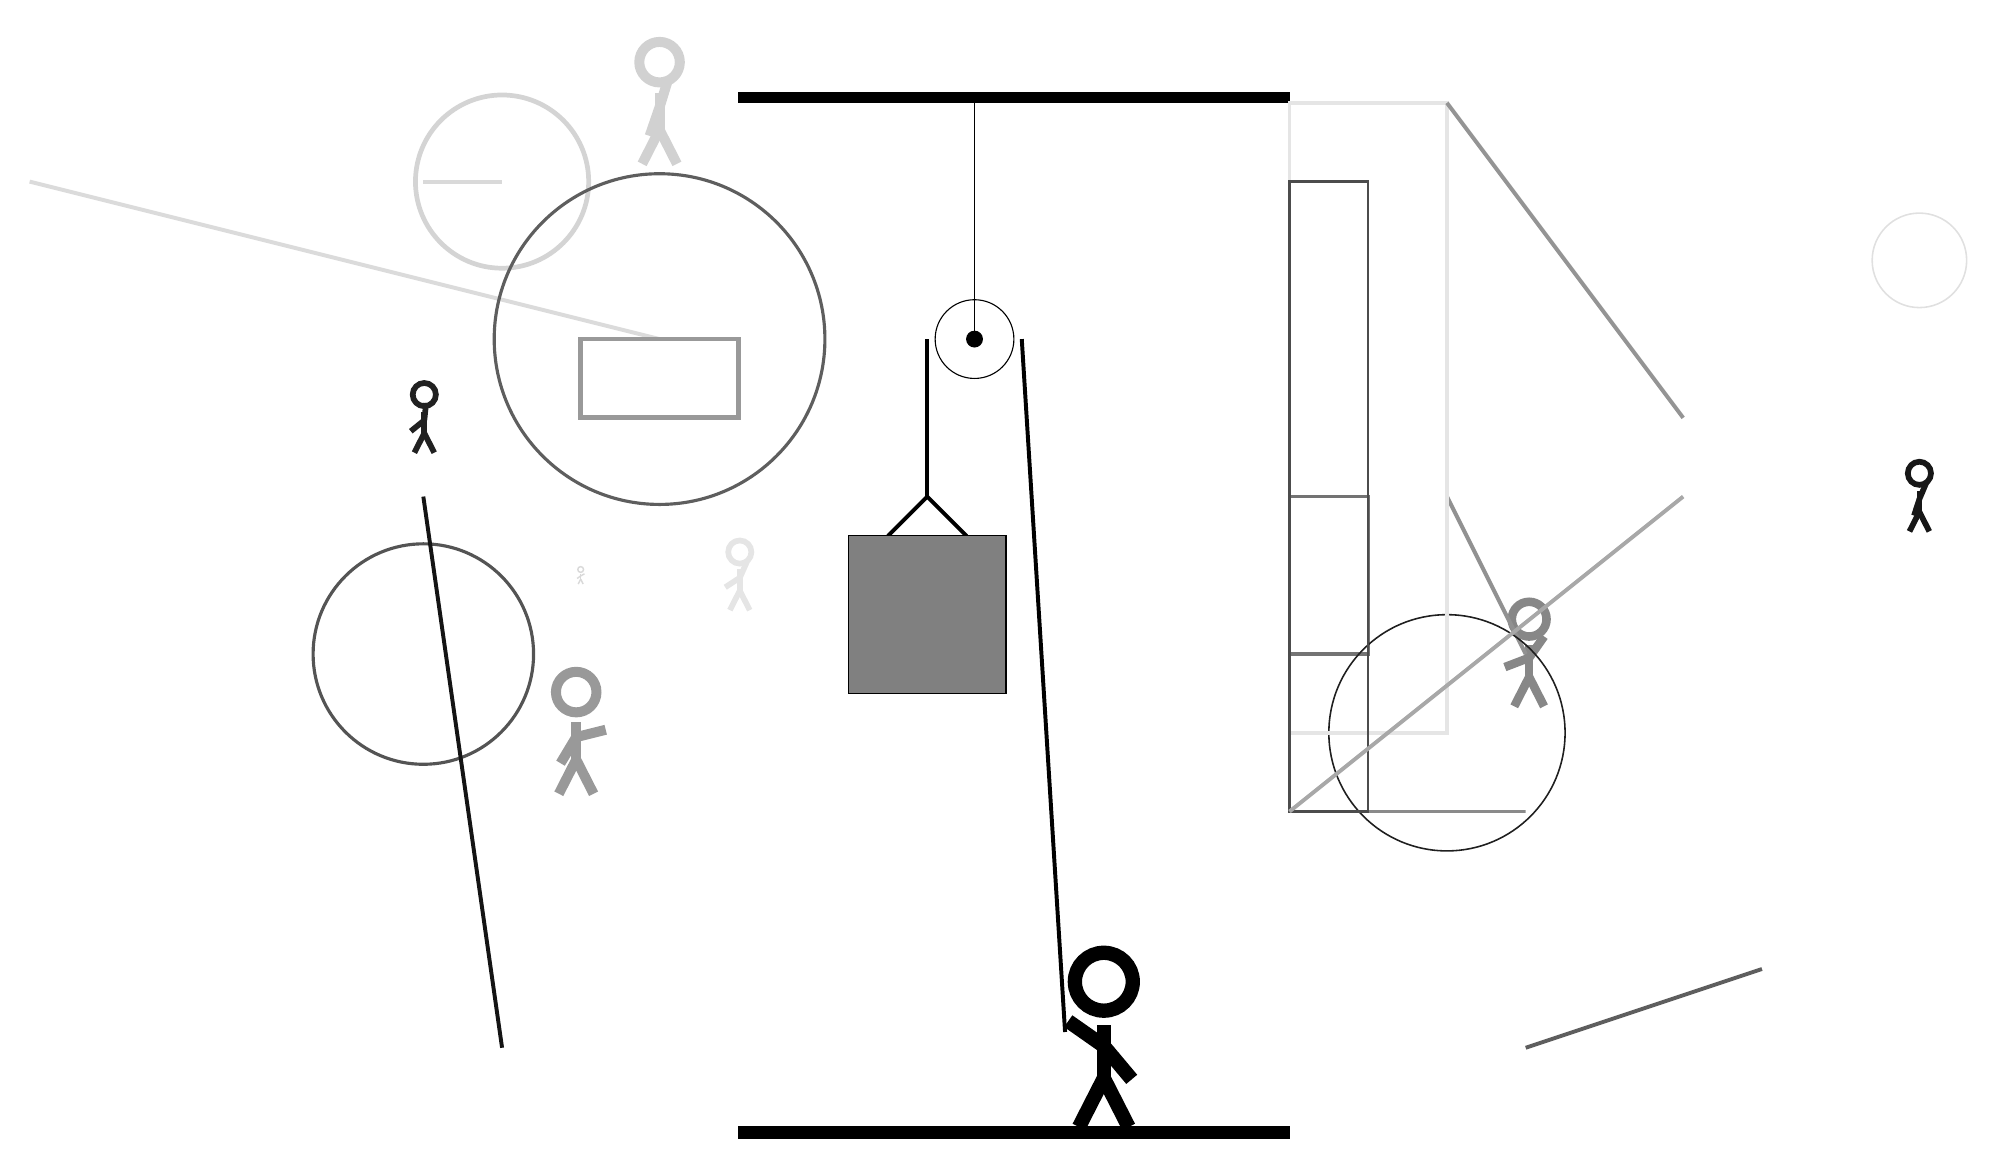
\begin{tikzpicture}
		%%%%% START %%%%%
		
		\draw[fill=black] (-2, 10) rectangle (5, 10.125);
		
		\draw (1, 7) circle (0.5);
		\draw[fill=black] (1, 7) circle (0.1);
		\draw (1, 10) -- (1, 7);
		
		\draw[line width=0.4mm, color=black!55] (5, 3) rectangle (6, 5);
		
		\node[line width=0.2mm, color=black!15] at (-4, 4) {\Strichmaxerl[1][36][29]};
		\node[line width=0.2mm, color=black!18] at (-3, 10) {\Strichmaxerl[7][71][73]};
		\node[line width=0.3mm, color=black!91] at (13, 5) {\Strichmaxerl[4][72][67]};
		\draw [line width=0.6mm, color=black!17](-5, 9) circle (1.1);
		\node[line width=0.2mm, color=black!47] at (8, 3) {\Strichmaxerl[6][21][55]};
		\draw [line width=0.4mm, color=black!67](-6, 3) circle (1.4);
		
		\draw[line width=0.5mm, color=black!14](-3, 7) -- (-11, 9);
		\draw[line width=0.5mm, color=black!43](8, 3) -- (7, 5);
		\node[line width=0.7mm, color=black!10] at (-2, 4) {\Strichmaxerl[4][33][66]};
		\draw[line width=0.6mm, color=black!40] (-4, 6) rectangle (-2, 7);
		\draw[line width=0.5mm, color=black!63](8, -2) -- (11, -1);
		\draw [line width=0.2mm, color=black!88](7, 2) circle (1.5);
		
		\node[line width=0.6mm, color=black!87] at (-6, 6) {\Strichmaxerl[4][39][84]};
		\draw[line width=0.5mm, color=black!92](-5, -2) -- (-6, 5);
		\draw [line width=0.4mm, color=black!63](-3, 7) circle (2.1);
		
		\draw[line width=0.5mm, color=black!10] (7, 2) rectangle (5, 10);
		\draw[line width=0.3mm, color=black!46] (5, 1) rectangle (8, 1);
		\node[line width=0.6mm, color=black!40] at (-4, 2) {\Strichmaxerl[7][59][14]};
		\draw [line width=0.2mm, color=black!12](13, 8) circle (0.6);
		\draw[line width=0.5mm, color=black!15](-6, 9) -- (-5, 9);
		\draw[line width=0.3mm, color=black!70] (6, 1) rectangle (5, 9);
		\draw[line width=0.5mm, color=black!42](7, 10) -- (10, 6);
		\draw[line width=0.5mm, color=black!34](10, 5) -- (5, 1);
		
		\draw[line width=0.5mm] (-0.1, 4.5) -- (0.4, 5.0) -- (0.9, 4.5);
		\draw[fill=black!50] (-0.6, 4.5) rectangle (1.4, 2.5);
		
		\draw[line width=0.5mm] (0.4, 7) -- (0.4, 5.0);
		\centerarc[line width=0.5mm](1, 7)(0:180:0.6);
		\draw[line width=0.5mm](1.6, 7) -- (2.15, -1.8);
		
		\node at (2.6, -1.9) {\Strichmaxerl[10][-35][-50]};
		
		\draw[fill=black] (-2, -3) rectangle (5, -3.15);
		
		%%%%% END %%%%%
	\end{tikzpicture}
\end{document}